\ifdefined\ishandout
  \documentclass[handout]{beamer}
\else
  \documentclass{beamer}
\fi

\usetheme{boxes}
\definecolor{beamer@structure@color}{rgb}{0,0,0}

\usecolortheme{structure}

\setbeamertemplate{footline}[frame number]
\setbeamertemplate{frametitle}{\color{black}
\def\myhrulefill{\leavevmode\leaders\hrule height 1pt\hfill\kern 0pt}
\headingfont\insertframetitle\par\vskip-8pt\myhrulefill}

\newcommand{\personality}[1]{{\bf #1}}

\usepackage[all]{xy}
\usepackage{cancel}

\newcommand*{\longhookrightarrow}{\ensuremath{\lhook\joinrel\relbar\joinrel\rightarrow}}
\newcommand{\dirlim}{\varinjlim}
\newcommand{\homot}{\simeq}
\newcommand{\NN}{\mathbb{N}}
\newcommand{\ZZ}{\mathbb{Z}}
\newcommand{\QQ}{\mathbb{Q}}
\newcommand{\RR}{\mathbb{R}}
\newcommand{\CC}{\mathbb{C}}
\newcommand{\FF}{\mathbb{F}}
\newcommand{\isom}{\cong}
\DeclareMathOperator{\SL}{SL}
\DeclareMathOperator{\Sp}{Sp}
\DeclareMathOperator{\Cl}{Cl}
\renewcommand{\O}{\mathcal{O}}
\newcommand{\dfn}{\mathrel{\mathop:}=}
\DeclareMathOperator{\ord}{ord}
\DeclareMathOperator{\rk}{rk}
\DeclareMathOperator{\Res}{Res}
\DeclareMathOperator{\Spec}{Spec}

\setbeamertemplate{navigation symbols}{}

\usepackage{array}
\newcolumntype{x}[1]{>{\centering\hspace{0pt}}p{#1}}
\definecolor{shadecolor}{rgb}{0.89,0.89,0.89}
\usepackage{colortbl}

\newcommand{\term}{\textbf}

\renewcommand*\familydefault{\sfdefault}

\usepackage{mathspec}
\setsansfont[BoldFont={PT Sans Bold}, ItalicFont={PT Sans Italic}]{PT Sans}
\setmathrm[BoldFont={PT Sans Bold}, ItalicFont={PT Sans Italic}]{PT Sans}
\newfontfamily\headingfont[]{PT Sans Bold}

\begin{document}

% % % % % % % % % % % % % % % % % % % % % % % % % % % % % % % % % % % % % % % % % % % % %

\begin{frame}[noframenumbering]
  \headingfont
  \begin{center}
    {\huge Zeta-values from Euler\\
      to Weil-\'etale cohomology

    }

    \vspace{2em}

    {\large Alexey Beshenov}

    \vspace{0.20em}

    Universit\'e de Bordeaux / Universiteit Leiden

    \vspace{1em}

    {\large Advised by Baptiste Morin and Bas Edixhoven}

    \vspace{1em}

    {\tiny 15 May 2017, Leiden}

    \vspace{5em}

    \raisebox{+0.125cm}{
\includegraphics[width=2.5cm]{../u-bordeaux.pdf}}\hspace{0.9cm}
    \raisebox{+0.12cm}{
\includegraphics[width=2.25cm]{../leiden.pdf}}\hspace{0.9cm}
    \includegraphics[width=2.5cm]{../algant.mps}
  \end{center}
\end{frame}

% % % % % % % % % % % % % % % % % % % % % % % % % % % % % % % % % % % % % % % % % % % % % 

\begin{frame}
  \frametitle{Outline}

  \begin{itemize}
  \item<2-> XVIII century mathematics: $\sum_{n\ge 1} \frac{1}{n^{2k}}$.

  \item<3-> XIX century mathematics: $\zeta (s)$ and $\zeta_F (s)$.

  \item<4-> XX century mathematics: $\zeta_X (s)$.

  \item<5-> Algebraic $K$-theory.

  \item<6-> Motivic cohomology.

  \item<7-> Weil-\'etale cohomology.
  \end{itemize}

\end{frame}

% % % % % % % % % % % % % % % % % % % % % % % % % % % % % % % % % % % % % % % % % % % % % 

\begin{frame}
  \frametitle{Riemann zeta function before Riemann}

  \begin{itemize}
  \item<2-> \personality{Pietro Mengoli}, 1644, the ``Basel problem'':
    $\sum_{n \ge 1} \frac{1}{n^2} = 1 + \frac{1}{4} + \frac{1}{9} + \frac{1}{16} +\frac{1}{25} + \cdots = ?????$

  \item<3-> \personality{Euler}
    (\emph{``De summis serierum reciprocarum''}, 1740): $\frac{\pi^2}{6}$.

  \item<4-> In general (ibid.),\\
    $\sum_{n \ge 1} \frac{1}{n^{2k}} = (-1)^{k+1}\,B_{2k} \, \frac{2^{2k-1}}{(2k)!}\,\pi^{2k}$.

  \item<5-> Bernoulli numbers:\\
    $B_0 = 1$, $B_1 = \frac{1}{2}$, $B_2 = \frac{1}{6}$, $B_3 = 0$, $B_4 = -\frac{1}{30}$, $B_5 = 0$,\\
    $B_6 = \frac{1}{42}$, $B_7 = 0$, $B_8 = -\frac{1}{30}$, $B_9 = 0$, $B_{10} = \frac{5}{66}$, $\ldots$

    (\personality{Jacob Bernoulli}, \emph{``Ars Conjectandi''}, 1713).
    
  \item<6-> Faulhaber's formula:
    $\sum_{1\le i\le n} i^k = \frac{1}{k+1}\,\sum_{0 \le i \le k} {k+1\choose i}\,B_i\,n^{k+1-i}$

    (\personality{Johann Faulhaber}, \emph{``Academia Algebr\ae''}, 1631;
    Bernoulli, 1713).
  \end{itemize}
\end{frame}

% % % % % % % % % % % % % % % % % % % % % % % % % % % % % % % % % % % % % % % % % % % % % 

\begin{frame}
  \frametitle{Riemann zeta function}

  \personality{Riemann}, \emph{``Ueber die Anzahl der Primzahlen unter einer
    gegebenen Gr\"{o}sse''} (1859):

  \begin{itemize}
  \item<2-> $\zeta (s) \dfn \sum_{n \ge 1} \frac{1}{n^s} \quad\quad (\operatorname{Re} s > 1)$.

  \item<3-> \personality{Euler}
    (\emph{``Vari\ae{} observationes circa series infinitas''}, 1744):
    $= \prod_{p\text{ prime}} \frac{1}{1 - p^{-s}}$.

  \item<4-> Meromorphic continuation to $\CC$ with one simple pole at $s = 1$.

  \item<5-> Functional equation
    $$\zeta (1-s) = 2\,(2\pi)^{-s}\,\Gamma (s) \, \cos \left(\frac{\pi s}{2}\right)\,\zeta(s).$$
  \end{itemize}

  \begin{itemize}
  \item<6-> (Trivial) simple zeros at $s = -2, -4, -6, \ldots$

  \item<7-> Euler's calculation
    $\zeta (2k) = (-1)^{k+1}\,B_{2k} \, \frac{2^{2k-1}}{(2k)!}\,\pi^{2k}$
    becomes
    $$\zeta (-n) = -\frac{B_{n+1}}{n+1} \text{ for } n = 1,2,3,4,\ldots$$
  \end{itemize}
\end{frame}

% % % % % % % % % % % % % % % % % % % % % % % % % % % % % % % % % % % % % % % % % % % % % 

\begin{frame}
  \begin{center}
    \includegraphics[width=10cm]{zeta-pos.mps}
  \end{center}
\end{frame}

% % % % % % % % % % % % % % % % % % % % % % % % % % % % % % % % % % % % % % % % % % % % % 

\begin{frame}
  \begin{center}
    \includegraphics[width=10cm]{zeta.mps}
  \end{center}
\end{frame}

% % % % % % % % % % % % % % % % % % % % % % % % % % % % % % % % % % % % % % % % % % % % % 

\begin{frame}
  \frametitle{Riemann zeta function at positive odd integers}

  \begin{itemize}
  \item<2-> \personality{Roger Ap\'ery}, 1977: $\zeta (3) = 1.2020569...$ is
    irrational.

  \item<3-> \personality{Tanguy Rivoal}, 2000: infinitely many irrationals
    $\zeta (2k+1)$.

  \item<4-> \personality{Wadim Zudilin}, 2001: at least one irrational among\\
    $\zeta(5), ~ \zeta(7), ~ \zeta(9), ~ \zeta(11)$ (which one?)

  \item<5-> Conjecture: $\zeta (2k+1)$ are transcendental, algebraically
    independent.
  \end{itemize}
\end{frame}

% % % % % % % % % % % % % % % % % % % % % % % % % % % % % % % % % % % % % % % % % % % % % 

\begin{frame}
  \frametitle{Dedekind zeta function: definition}

  \begin{itemize}
  \item<2-> $F/\QQ$~--- number field, $\O_F \dfn \text{the ring of integers}$.

  \item<3-> \personality{Dedekind}, appendix to Dirichlet's ``Vorlesungen \"uber
    Zahlentheorie'' (1863):

    \[ \zeta_F (s) \dfn \sum_{\substack{\mathfrak{a} \subset \O_F \\ \mathfrak{a} \ne 0}} \frac{1}{N_{F/\QQ} (\mathfrak{a})^s} =
      \prod_{\substack{\mathfrak{p} \subset \O_F \\ \text{prime}}} \frac{1}{1 - N_{F/\QQ} (\mathfrak{p})^{-s}}.
      \quad\quad (\operatorname{Re} s > 1) \]

  \item<4-> Note: $\zeta_\QQ (s) = \zeta (s)$.
  \end{itemize}
\end{frame}

% % % % % % % % % % % % % % % % % % % % % % % % % % % % % % % % % % % % % % % % % % % % % 

\begin{frame}
  \frametitle{Dedekind zeta function: functional equation}

  \begin{itemize}
  \item<2-> \personality{Hecke}, \emph{``\"Uber die Zetafunktion beliebiger
      algebraischer Zahlk\"orper''}, 1917: meromorphic continuation with simple
    pole at $s=1$; functional equation
    \begin{multline*}
      $$\zeta_F (1-s) = |\Delta_F|^{s - 1/2} \, \left(\cos \frac{\pi s}{2}\right)^{r_1+r_2} \, \left(\sin \frac{\pi s}{2}\right)^{r_2} \\
      \left(2 \, (2\pi)^{-s} \, \Gamma (s)\right)^d\,\zeta_F (s),
    \end{multline*}
    where
    $r_1 \dfn \text{real places}$, $r_2 \dfn \text{pairs of complex places}$;

    $d \dfn [F : \QQ] = r_1 + 2\,r_2$ and $\Delta_F \dfn \text{discriminant}$.

  \item<4-> (Trivial) zeros:
  \end{itemize}

  \onslide<4->{\small
    \begin{center}
      \begin{tabular}{rcccx{3em}cx{3em}cx{3em}cc}
        \hline
        $s\colon$ & $0$ & $-1$ & $-2$ & $-3$ & $-4$ & $-5$ & $\cdots$\tabularnewline
        \hline
        order: & $r_1+r_2-1$ & $r_2$ & $r_1+r_2$ & $r_2$ & $r_1+r_2$ & $r_2$ & $\cdots$ \tabularnewline
        \hline
      \end{tabular}
    \end{center}}
\end{frame}

% % % % % % % % % % % % % % % % % % % % % % % % % % % % % % % % % % % % % % % % % % % % % 

\begin{frame}
  \frametitle{Class number formula}

  \personality{Dirichlet}, \emph{``Recherches sur diverses applications de l'analyse infinit\'esimale \`a la th\'eorie des nombres''} (1839);\\
  * \personality{Gauss}, \emph{``Disquisitiones Arithmetic\ae''} (1801):

  \begin{itemize}
  \item<2-> Pole at $s = 1$:

    $$\lim_{s\to 1} (s-1)\,\zeta_F (s) = \frac{2^{r_1}\,(2\pi)^{r_2}\,\#\Cl (F)}{\#\mu_F \cdot \sqrt{|\Delta_F|}}\,R_F,$$
    where $\Cl (F)$~--- class group; $\mu_F \subset \O^\times_F$~--- roots of unity;\\
    $R_F$~--- Dirichlet regulator.

  \item<3-> Zero at $s = 0$:
    $$\lim_{s\to 0} s^{-(r_1 + r_2 - 1)}\,\zeta_F (s) = -\frac{\#\Cl (F)}{\#\mu_F}\,R_F.$$
  \end{itemize}
\end{frame}

% % % % % % % % % % % % % % % % % % % % % % % % % % % % % % % % % % % % % % % % % % % % % 

\begin{frame}
  \frametitle{Values of the Dedekind zeta function}

  \begin{itemize}
  \item<2-> If $F$ is totally real ($r_2 = 0$), then $\zeta_F (-n) \ne 0$
    odd $n$.

  \item<3-> ``Siegel--Klingen theorem'', 1961: $\zeta_F (-n) \in \QQ$.

  \item<4-> \personality{G\"unter Harder}, ``A Gauss--Bonnet formula for
    discrete arithmetically defined groups'', 1971:
    $$\chi (\Sp_{2n} (\O_F)) = \frac{1}{2^{n\,(d-n)}} \, \prod_{1\le i\le n} \zeta_F (1-2n).$$

  \item<5-> Example: $F = \QQ$, $n = 1$, $\Sp_2 = \SL_2$,
    $$\chi (\SL_2 (\ZZ)) = -\frac{1}{12} = -\frac{B_2}{2} = \zeta (-1)$$
    (``orbifold Euler characteristic'' of $\mathcal{H}/\SL_2 (\ZZ)$).
  \end{itemize}
\end{frame}

% % % % % % % % % % % % % % % % % % % % % % % % % % % % % % % % % % % % % % % % % % % % % 

\begin{frame}
  \frametitle{Zeta function of a scheme}

  \begin{itemize}
  \item<2-> $X \to \Spec \ZZ$~--- arithmetic scheme (separated, of finite type).

  \item<3-> $\zeta_X (s) \dfn \prod_{x\in X_0} \frac{1}{1 - N (x)^{-s}}. \quad\quad (\operatorname{Re} s > \dim X)$.

    $X_0 \dfn \text{closed points}$; $N (x) \dfn \#\text{residue field at }x$.

  \item<4-> Note: $\zeta_{\Spec\ZZ} (s) = \zeta (s)$ and $\zeta_{\Spec\O_F} (s) = \zeta_F (s)$.

  \item<5-> Conjecture (!): meromorphic continuation and a functional equation
    $\zeta_X (s) \leftrightarrow \zeta_X (\dim X - s)$.

  \item<6-> Special values may be studied via\\
    $K$-theory $K_n (X)$ or motivic cohomology $H^i (X, \ZZ (n))$.
  \end{itemize}
\end{frame}

% % % % % % % % % % % % % % % % % % % % % % % % % % % % % % % % % % % % % % % % % % % % % 

\begin{frame}
  \frametitle{Algebraic K-theory}

  \begin{itemize}
  \item<2-> Input: an ``exact category'' $\mathcal{C}$.

    Examples: $\textbf{VB} (X)$ and $R\textbf{-Proj}_{fg} \simeq \textbf{VB} (\Spec R)$.

  \item<3-> \personality{Grothendieck}, 1957\\
    (work on [Grothendieck--Hirzebruch]--Riemann--Roch):
    $$K_0 (\mathcal{C}) \dfn \frac{\ZZ \left<\text{isomorphism classes of objects of }\mathcal{C}\right>}{[B] = [A]+[C]\text{ for each s.e.s. } 0\to A\to B\to C\to 0}.$$

  \item<4-> \personality{Quillen}, 1973:

    \begin{align*}
      K_0 (\mathcal{C}) & \isom \pi_1 (BQ\mathcal{C}, 0),\\
      K_n (\mathcal{C}) & \dfn \pi_{n+1} (BQ\mathcal{C}, 0);
    \end{align*}

    $Q$~--- Quillen's ``$Q$-construction'',\\
    $B$~--- geometric realization of the nerve.
  \end{itemize}
\end{frame}

% % % % % % % % % % % % % % % % % % % % % % % % % % % % % % % % % % % % % % % % % % % % % 

\begin{frame}
  \begin{center}
    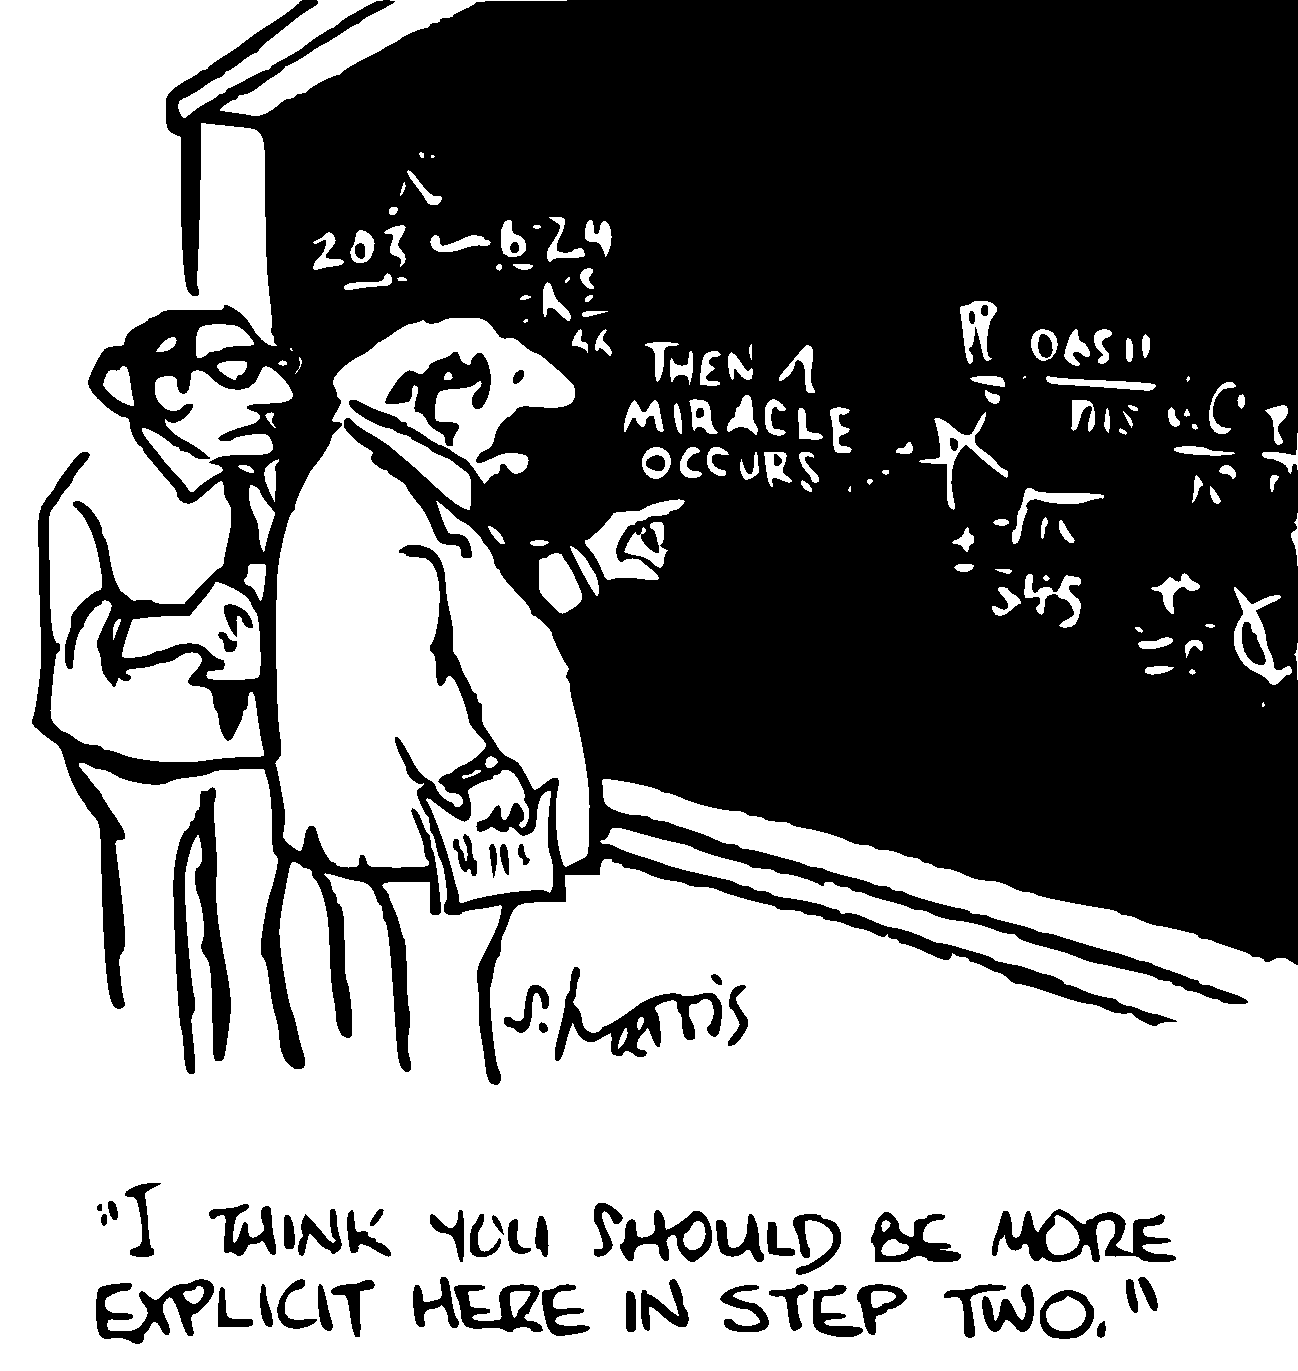
\includegraphics[width=8cm]{miracle.pdf}

    {\small\color[rgb]{0.6,0.6,0.6} \copyright{} Sidney Harris}
  \end{center}
\end{frame}

% % % % % % % % % % % % % % % % % % % % % % % % % % % % % % % % % % % % % % % % % % % % % 

\begin{frame}
  \frametitle{Some of the few known calculations}

  \begin{itemize}
  \item<2-> \personality{Quillen}, 1972:

    \begin{align*}
      K_0 (\FF_q) & \isom \ZZ,\\
      K_{2n} (\FF_q) & = 0,\\
      K_{2n-1} (\FF_q) & \isom \ZZ/(q^n - 1)\ZZ.
    \end{align*}

  \item<3-> Note: $\# K_{2n-1} (\FF_q) = -\zeta_{\FF_q} (-n)^{-1}$.

  \item<4-> \personality{Quillen}, 1973: $K_n (\O_F)$ are finitely generated.

  \item<5-> \personality{Armand Borel}, 1974:

    $$\rk K_n (\O_F) = \begin{cases}
      0, & n = 2k,\\
      r_1+r_2, & n = 4k + 1,\\
      r_2, & n = 4k -1.
    \end{cases} \quad\quad (k > 0)$$

  \item<6-> Note: $\rk K_{2n+1} (\O_F) = \text{order of zero of }\zeta_F (s)\text{ at }s=-n.$
  \end{itemize}
\end{frame}

% % % % % % % % % % % % % % % % % % % % % % % % % % % % % % % % % % % % % % % % % % % % % 

\begin{frame}
  \frametitle{Torsion in the K-theory of $\ZZ$}

  \begin{itemize}
  \item<2-> \personality{Milnor}, 1971: $K_2 (\ZZ) \isom \ZZ/2\ZZ$.

  \item<3-> \personality{Lee}, \personality{Szczarba}, 1976:
    $K_3 (\ZZ) \isom \ZZ/48 \ZZ$.

  \item<4-> \personality{Rognes}, 2000: $K_4 (\ZZ) = 0$.

  \item<5-> \personality{Elbaz-Vincent}, \personality{Gangl},
    \personality{Soul\'e}, 2002: $K_5 (\ZZ) \isom \ZZ$.

  \item<6-> Using the Bloch--Kato conjecture (\personality{Voevodsky},
    \personality{Rost}, ...):
  \end{itemize}

  \onslide<6->{\small
    \begin{center}
      \begin{tabular}{rx{1.8cm}x{1.8cm}x{1.8cm}x{1.8cm}}
        \hline
        $n\colon$ & 2 & 3 & 4 & 5 \tabularnewline
        $K_n (\ZZ)\colon$ & $\ZZ/2\ZZ$ & $\ZZ/48\ZZ$ & $0$ & $\ZZ$ \tabularnewline
        \hline
        $n\colon$ & 6 & 7 & 8 & 9 \tabularnewline
        $K_n (\ZZ)\colon$ & $0$ & $\ZZ/240\ZZ$ & $(0?)$ & $\ZZ\oplus\ZZ/2\ZZ$ \tabularnewline
        \hline
        $n\colon$ & 10 & 11 & 12 & 13 \tabularnewline
        $K_n (\ZZ)\colon$ & $\ZZ/2\ZZ$ & $\ZZ/1008\ZZ$ & $(0?)$ & $\ZZ$ \tabularnewline
        \hline
        $n\colon$ & 14 & 15 & 16 & 17 \tabularnewline
        $K_n (\ZZ)\colon$ & $0$ & $\ZZ/480\ZZ$ & $(0?)$ & $\ZZ\oplus\ZZ/2\ZZ$ \tabularnewline
        \hline
        $n\colon$ & 18 & 19 & 20 & 21 \tabularnewline
        $K_n (\ZZ)\colon$ & $\ZZ/2\ZZ$ & $\ZZ/528\ZZ$ & $(0?)$ & $\ZZ$ \tabularnewline
        \hline
        $n\colon$ & 22 & 23 & 24 & 25 \tabularnewline
        $K_n (\ZZ)\colon$ & $\ZZ/691\ZZ$ & $\ZZ/65\,520\ZZ$ & $(0?)$ & $\ZZ\oplus\ZZ/2\ZZ$ \tabularnewline
        \hline\tabularnewline
      \end{tabular}
    \end{center}}
\end{frame}

% % % % % % % % % % % % % % % % % % % % % % % % % % % % % % % % % % % % % % % % % % % % % 

\begin{frame}
  \frametitle{Lichtenbaum's conjecture}

  \begin{itemize}
  \item<2-> Easy: $K_0 (\O_F) \isom \Cl (F) \oplus \ZZ$.

  \item<3-> Not-so-easy (\personality{Bass}, \personality{Milnor},
    \personality{Serre}, 1967): $K_1 (\O_F) \isom \O_F^\times$.

  \item<4-> Dirichlet's unit theorem:
    $\O_F^\times \isom \ZZ^{r_1+r_2-1} \oplus \mu_F$.

  \item<5-> Class number formula:
    $$\lim_{s\to 0} s^{-(r_1 + r_2 - 1)}\,\zeta_F (s) = -\frac{\#K_0 (\O_F)_{tors}}{\#K_1 (\O_F)_{tors}}\,R_F.$$

  \item<6-> \personality{Lichtenbaum}, 1973:
    $$\lim_{s\to n} (n-s)^{-\mu_n}\,\zeta_F (-s) = \pm 2^{?}\,\frac{\#K_{2n} (\O_F)}{\#K_{2n+1} (\O_F)_{tors}}\,R_{F,n}.$$

    $R_{F,n}$~--- ``higher regulators'' (Borel, Beilinson).

  \item<7-> Example: $\zeta (-1) = -\frac{B_2}{2} = -\frac{1}{12}$,
    $\frac{\# K_2 (\ZZ)}{\# K_3 (\ZZ)} = \frac{\# \ZZ/2}{\# \ZZ/48} = \frac{1}{24}$.

  \item<8-> Example:
    $\zeta (-11) = -\frac{B_{12}}{12} = \frac{691}{12\cdot 2730} = \frac{691}{2^3\cdot 3^2\cdot 5\cdot 7\cdot 13}$,
    $\frac{\# K_{22} (\ZZ)}{\# K_{23} (\ZZ)} = \frac{691}{65520} = \frac{691}{2^4\cdot 3^2\cdot 5\cdot 7\cdot 13}$.
  \end{itemize}
\end{frame}

% % % % % % % % % % % % % % % % % % % % % % % % % % % % % % % % % % % % % % % % % % % % % 

\begin{frame}
  \frametitle{Motivic cohomology}

  \begin{itemize}
  \item<2-> \personality{Bloch}, 1986: complexes of Zariski / \'etale sheaves
    $\ZZ (n)$.

    % \item Example: $\ZZ (0) \isom \ZZ$ for $X$ normal.
    % \item $\ZZ (1) \isom \mathbb{G}_m [-1]$ for $X$ smooth of f.t. / $\FF_q$
    %   or a Dedekind ring.

  \item<3-> $H^i (X_\text{Zar}, \ZZ (n))$, $H^i (X_\text{\'et}, \ZZ (n))$~---
    (hyper)cohomology groups.

  \item<4-> Finite generation, boundedness for arithmetic $X$: conjectures.

  \item<5-> Possible motivation (no pun intended):
    $$E_2^{pq} = H^p (X, \ZZ (q)) \Longrightarrow K_{2q-p} (X),$$
    similar to the Atiyah--Hirzebruch spectral sequence.

  \item<6-> $H^i (X_\text{\'et}, \ZZ (n))$ might be better for studying the
    zeta-values.
  \end{itemize}
\end{frame}

% % % % % % % % % % % % % % % % % % % % % % % % % % % % % % % % % % % % % % % % % % % % % 

\begin{frame}
  \frametitle{Weil-\'etale cohomology (Lichtenbaum, 2005)}

  \onslide<2->{For an arithmetic scheme $X$ there should (!) exist abelian
    groups $H^i_{W,c} (X, \ZZ (0))$ and real vector spaces
    $H^i_W (X,\widetilde{\RR} (0))$, $H^i_{W,c} (X,\widetilde{\RR} (0))$ such
    that}

  \begin{enumerate}
  \item<3-> $H^i_{W,c} (X,\ZZ (0))$ are f.g., almost all zero.

  \item<4-> $H^i_{W,c} (X, \ZZ (0)) \otimes \RR \xrightarrow{\isom} H^i_{W,c} (X,\widetilde{\RR} (0))$.

  \item<5-> For a canonical class $\theta \in H^1_W (X,\widetilde{\RR} (0))$
    $$\cdots \xrightarrow{\cup\theta} H^i_{W,c} (X,\widetilde{\RR} (0)) \xrightarrow{\cup\theta} H^{i+1}_{W,c} (X,\widetilde{\RR} (0)) \xrightarrow{\cup\theta} \cdots$$
    a bounded acyclic complex of f.d. vector spaces.

  \item<6-> $\ord_{s=0} \zeta (X,s) = \sum_{i\ge 0} (-1)^i \cdot i \cdot \rk_\ZZ H^i_{W,c} (X, \ZZ (0))$.

  \item<7-> $\ZZ \cdot \lambda (\zeta^* (X,0)^{-1}) = \bigotimes_{i\in\ZZ} \det_\ZZ H^i_{W,c} (X,\ZZ (0))^{(-1)^i}$,

    where
    $\lambda\colon \RR \xrightarrow{\isom} \left(\bigotimes_{i\in\ZZ} \det_\ZZ H^i_{W,c} (X,\ZZ (0))^{(-1)^i}\right)\otimes \RR$.
  \end{enumerate}
\end{frame}

% % % % % % % % % % % % % % % % % % % % % % % % % % % % % % % % % % % % % % % % % % % % % 

\begin{frame}
  \frametitle{Weil-\'etale cohomology}

  \begin{itemize}
  \item<2-> \personality{Geisser}, 2004; \personality{Lichtenbaum}, 2005:
    construction of $H^i_{W,c} (X, \ZZ (n))$ for smooth varieties over finite
    fields.

  \item<3-> \personality{Lichtenbaum}, 2009: $H^i_{W,c} (X, \ZZ (0))$ for
    $X = \Spec \O_F$.

  \item<4-> \personality{Morin}, 2012: $H^i_{W,c} (X, \ZZ (0))$\\
    for proper regular arithmetic schemes.

  \item<5-> \personality{Flach}, \personality{Morin}, 2016:
    $H^i_{W,c} (X, \ZZ (n))$ for $n\in \ZZ$ \\
    for proper regular arithmetic schemes.

  \item<6-> My thesis, work in progress: $H^i_{W,c} (X, \ZZ (n))$

    \begin{itemize}
    \item for any arithmetic scheme (makes things harder)
    \item and $n = -1,-2,-3,-4,\ldots$ (makes things easier)
    \end{itemize}

  \item<7-> Construction via the cycle complexes $\ZZ (n)$, following Flach and
    Morin (input: conjectures on finite generation and boundedness).
  \end{itemize}
\end{frame}

% % % % % % % % % % % % % % % % % % % % % % % % % % % % % % % % % % % % % % % % % % % % % 

\begin{frame}[plain]
  \headingfont

  \vspace{\fill}

  \begin{center}
    {\huge Thank you!}
  \end{center}

  \vspace{\fill}
\end{frame}

\end{document}
